\section{Data} \label{sec:Data}

The empirical specification from Sect.~\ref{sec:Specification} (Eq.~\ref{eq:specification}) implies that we need data on rewards credit cards point multipliers, point values, benefits, and fees, as well as budget data for our credit card users.

\subsection{Credit Card Data} \label{subsec:CreditCardData}

There are many websites writing about rewards credit cards, their perks, and points structure. 
I mainly used the website allcards.com%
\footnote{\url{https://www.allcards.com} (accessed between June 3--9, 2024).}
to manually scrape the information on point multipliers and their caps (limits) from the most popular rewards credit cards from the seven major banks (American Express, Chase, Bank of America, Citi, Capital One, US Bank, and Wells Fargo). 
The bank websites were used to find some missing information, if needed. 
This resulted in a list of 28 unique credit cards. 
However, some of the cards have a ``custom'' bonus reward category that can be chosen by the user (e.g. 5x points on groceries, or gas, or home improvement up to \$6000 per year). 
These cards were treated as a separate credit card for each bonus category, bringing our total number of cards to 38. 

I ignored credit cards that are dedicated to users of very specific stores, hotels, or airlines, as well as cards with rather exotic, or variable, reward categories (such as ``3x points on all mobile wallet payments'', or ``5x points on quarterly changing categories''), since these categories are impossible to map to our budget categories that will be discussed in the next section. 
The results on total benefits should therefore be considered \emph{lower limits}, as there are many cards that can bring additional benefits to loyal users of certain brands.
 
A list of 18 common card spending categories was taken from the website cardpointers.com,%
\footnote{\url{https://www.cardpointers.com/app/} (accessed between June 3--9, 2024).}
with the modification of removing ``warehouse clubs'' and ``ride sharing'', and adding ``streaming'' and ``travel (other)'', to facilitate a mapping of all the items on our budget to a spending category (see Sect.~\ref{subsec:UserData}). The final list of all the categories can be found in the first column of Table~\ref{tab:BudgetExtended} in the Data Appendix.

For the base and travel values of the credit card points, I used the table from the \citet{nerdwallet:2024} website. 
These values are shown in Table~\ref{tab:PointValues} in the Data Appendix and will be used for the sensitivity analysis and Monte Carlo simulation.
Point values can be subjective, however, so for the \sR\ \textsf{Shiny} recommendation app, I foresee an update in the near future, making the point values adjustable by the user. 

Annual fees were also collected for all the cards in the dataset, as well as an estimate for the static benefits. 
We refer the reader to the Data Appendix on page~\pageref{app:Data} for a more detailed description of how the static benefits were handled. 
The appendix also shows an exerpt of the final credit card dataset in Fig.~\ref{fig:CreditCardsCSV}.


\subsection{User Data} \label{subsec:UserData}

For our credit card users we need a vector $\mathbf{x}$ with the amount of spend for each of the 18 spending categories. 
In the credit card portfolio recommendation app, the user can specify a personal yearly budget. 
For our analysis of how the optimal portfolios behave for different user preferences and budgets, however, we need realistic estimates of the average spending of Americans, since regulations and privacy concerns make obtaining actual spending data practically impossible for researchers outside of the banking sector.
I will therefore use the 2022 Consumer Expenditure Survey (CES) from the Bureau of Labor Statistics \citep{bls:2023}.

According to the CES, the average annual expenditures in 2022 were \$72,967 (after savings), from an average income before taxes of \$94,003.
To approximate the amount that can be spend on credit cards, I subtracted from the \$72,967 the expenses on shelter (such as mortgage, rent, property taxes), vehicle purchases, health insurance, education, cash contributions, personal insurance, and pensions.
The resulting budget totals to \$38,576 or 41 percent of the average gross income. 
The remaining CES items were then mapped to the credit card spending categories according to Table~\ref{tab:BudgetExtended} in the Data Appendix. Note that some items were split 50/50 over multiple credit card categories, to make sure that all the categories were populated with some reasonable spend. For example, I assumed that the CES item ``Apparel and services'' is split 50/50 between the ``Online shopping'' and ``Department store'' credit card categories. 

The CES also provides expenditures separated by nine income levels. 
I have repeated the above construction of the average budget also for these nine income bins separately, and saved the results in the file \texttt{BudgetIncome.csv}. The percentages spend per credit card category are also shown in Table~\ref{tab:BudgetIncome} in the Data Appendix.
For a given user's income (before taxes), the corresponding income bin from this table is used to calculate the average budget, namely by multiplying the gross income by the percentage spend in each category. 
Our algorithm will then predict the total credit cards benefit as a function of income, as well as $\eta$, $\theta$, and the number of credit cards $K$ (see Sect.~\ref{sec:Specification}). 

\begin{figure}[t!h]
    \begin{center}
    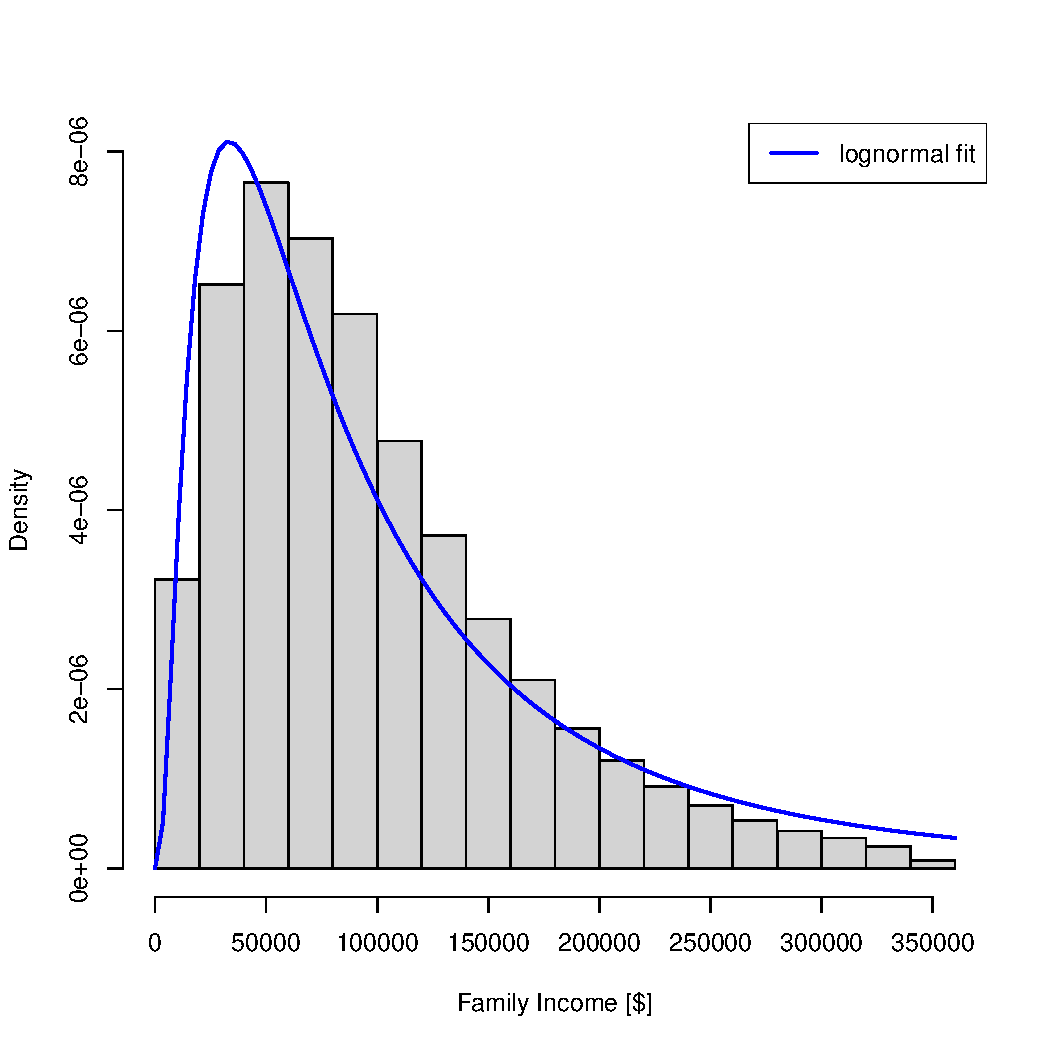
\includegraphics[width=0.6\textwidth]{../Figures/IncomeDistribution.pdf}
    \caption{2022 Florida income distribution from the BLS ACS (microdata sample of 57,005 observations, truncated at \$350,000 for this visualization).}
    \label{fig:IncomeDistribution}
    \end{center}
\end{figure}

A Monte Carlo simulation should give a reasonable estimate of the average net benefit and standard deviation for Americans who use an optimized credit card portfolio. 
For this simulation we need to sample (with replacement) income, $\eta$, $\theta$, and $K$ from realistic distributions. 
For the income distribution I used 2022 ``Family income'' (variable FINCP) from the BLS American Community Survey (ACS) Microdata tables, selecting all counties in Florida (resulting in 57,005 individual incomes).%
\footnote{\url{https://data.census.gov/mdat/\#/search?ds=ACSPUMS1Y2022} (accessed June 25,2024).}
This income distribution is shown in Fig.~\ref{fig:IncomeDistribution} and approximates a lognormal distribution.
User preferences $\eta$ and $\theta$ are sampled from a uniform distribution between 0--1, and $K$ is sampled from a uniform distribution between 1--8.
